\documentclass[conference]{IEEEtran}
\IEEEoverridecommandlockouts
% Based on the IEEE Conference Template (Overleaf). Compile with pdfLaTeX (Overleaf default) or tectonic.
\usepackage[T1]{fontenc}
\usepackage{cite}
\usepackage{amsmath,amssymb,amsfonts}
\usepackage{algorithm}
\usepackage{algpseudocode}
\usepackage{graphicx}
\usepackage{textcomp}
\usepackage{xcolor}
\usepackage{booktabs}
\usepackage{placeins}
\usepackage{url}
\usepackage{tikz}
\usetikzlibrary{arrows.meta,positioning,fit,calc}
\usepackage[hidelinks]{hyperref}
\graphicspath{{figures/}}
\newcommand{\figref}[1]{Fig.~\ref{#1}}
\newcommand{\ind}[1]{\mathbf{1}\{#1\}}
\DeclareMathOperator{\clip}{clip}
\extrafloats{100}
\renewcommand{\topfraction}{0.9}\renewcommand{\dbltopfraction}{0.9}
\renewcommand{\textfraction}{0.07}\renewcommand{\floatpagefraction}{0.6}\renewcommand{\dblfloatpagefraction}{0.6}

\begin{document}

\title{MARS-O-RAN: Mission-Aware, Risk-Aware Elastic Network Slicing for Emergency Robotics in an O-RAN Digital Twin}

\author{\IEEEauthorblockN{Ishaan Jayaram Shetty}
\IEEEauthorblockA{\textit{Dept. of Electronics and Communication Engg.} \\
\textit{IIIT Dharwad}\\
Dharwad, India}
\and
\IEEEauthorblockN{Prashant Kumar}
\IEEEauthorblockA{\textit{Dept. of Electronics and Communication Engg.} \\
\textit{IIIT Dharwad}\\
Dharwad, India}
\and
\IEEEauthorblockN{Himanshu Kumar Sonkar}
\IEEEauthorblockA{\textit{Dept. of Electronics and Communication Engg.} \\
\textit{IIIT Dharwad}\\
Dharwad, India}
\and
\IEEEauthorblockN{Naman Kumar}
\IEEEauthorblockA{\textit{Dept. of Computer Science and Engg.} \\
\textit{IIIT Dharwad}\\
Dharwad, India}
}

\maketitle

\begin{abstract}
During an industrial emergency, robots, sensors, and responders share one radio cell, and the traffic that matters most changes as the mission advances. We study a gas-leak response in which five dependent tasks carry deadlines, freshness limits, and reliability targets, and we formulate slice allocation of physical resource blocks (PRBs) as a stochastic integer control problem with a tail-risk term. We propose MARS, a low-complexity controller that normalizes a mission-criticality score through a temperature-scaled softmax, damps changes toward the previous allocation, and holds allocations between task transitions with a slack-adaptive hold time. In a Python digital twin styled after the O-RAN control loop, MARS is compared with fixed, demand-proportional, and mission-aware heuristics, its earlier version, and a myopic optimizer with perfect knowledge of the current state, over 300 paired seeds and three operating points. Mission awareness raises the task-level success score from 0.361 (fixed slicing) to about 0.91 when all tasks are feasible. MARS matches the mission-aware heuristic and the optimizer on mission outcome at the benign and concurrent-task operating points while reconfiguring 84--87\% and 30--38\% less, respectively, during the mission. Under a severe incident it loses 2.9 percentage points of success ($p=0.015$). With concurrent tasks its criticality score splits PRBs between them much as the optimizer does. Edge-case sweeps show where MARS lags (scarce PRBs, extreme severity, tight deadlines, heavy workload), that task completion is compute-bound, and that an apparent budget paradox stems from fixed slice caps. All results come from a reproducible simulation, not from field measurements.
\end{abstract}

\begin{IEEEkeywords}
O-RAN, network slicing, emergency robotics, mission-aware resource allocation, edge computing, CVaR, digital twin.
\end{IEEEkeywords}

%=====================================================================
\section{Introduction}
A ground robot closing a leaking valve, a drone streaming camera frames to an edge server, responders viewing hazard overlays, and a field of gas sensors can all share one private cell during an industrial emergency. Their demands conflict, and which one deserves the spectrum depends on where the mission stands. Sensor uplink dominates while the leak is being located; control traffic matters more once the robot grips the valve. A slicing policy that looks only at instantaneous traffic volume cannot see this shift.

Open RAN makes application-driven control architecturally plausible. Its RAN Intelligent Controllers (RICs) run control loops at two time scales: a near-real-time RIC that acts on the base station over the E2 interface, and a non-real-time RIC that issues policies over A1 \cite{oranarch,oranwg3,polese}. A mission-aware slicing rule would sit in the near-real-time loop. We study the decision logic of such a rule in a Python digital twin; no E2 or A1 messages are exchanged and no RIC software is deployed.

We ask two questions. \emph{Can tying PRB shares to the mission's executable tasks improve task completion over fixed or demand-driven slicing, and at what reconfiguration cost?} And \emph{under which budgets, incident severities, deadlines, and workloads does the advantage disappear?}

\textbf{What drives the results.} We state up front which modelled mechanisms are active. (i) In the calibrated model, task completion is compute-bound: radio delivers a task's bits within about one second, while edge computation takes tens of seconds, so PRBs influence outcomes mainly through the edge share that is coupled to the radio share (Section~\ref{sec:service}). (ii) The Age-of-Information (AoI) limits and the finite-blocklength correction are modelled but never binding at the evaluated operating points. (iii) When the mission is a chain, only one task competes for resources at a time, so a criticality score can decide only \emph{which} slice is served; it matters for \emph{how much} only when tasks run concurrently, which motivates our concurrent-mission scenario. (iv) The CVaR term is part of the problem objective and of controller tuning; no controller enforces it as a constraint.

\textbf{Scope of baselines.} We compare against rule-based heuristics, the earlier version of our controller, and a one-step optimizer that knows the true service model and current state. We do not train a reinforcement-learning agent: the mission is a single non-stationary 300\,s episode, and an agent trained on the same synthetic model would mainly test the model rather than the slicing logic. The myopic optimizer instead indicates how close a model-free heuristic comes to a model-based decision rule.

\textbf{Contributions.}
\begin{enumerate}
\item A system model that couples a mission-task graph (chain and concurrent variants) to four slices, an analytical radio and edge service model, AoI freshness, and end-to-end reliability (Section~\ref{sec:model}).
\item A formulation of mission-aware slicing as a stochastic integer program with a CVaR term and reconfiguration cost (Section~\ref{sec:problem}).
\item MARS, a controller combining a temperature-scaled criticality softmax, damping toward the previous allocation, a slack-adaptive hold time, and a transition mode that suspends both stability mechanisms while a new task is being served (Section~\ref{sec:mars}).
\item A paired comparison with five baselines over 300 seeds at three operating points, with bootstrap confidence intervals, signed-rank tests, and an exact empirical CVaR estimator (Section~\ref{sec:results}).
\item Edge-case sweeps and ablations that locate where each controller fails and trace each failure to a model mechanism (Section~\ref{sec:edge}).
\end{enumerate}

%=====================================================================
\section{Related Work}
\textbf{Open RAN control and slicing.} The O-RAN specifications separate a near-real-time controller from a non-real-time one \cite{oranarch,oranwg3}, and Polese \emph{et al.} survey the interfaces and the learning-based applications proposed for both \cite{polese}. SafeSlice adds a safety layer so that a deep RL slicing agent respects cumulative and per-step latency limits \cite{safeslice}. Baguer \emph{et al.} show that slicing over Open RAN can sustain beyond-visual-line-of-sight drone operation \cite{bvlos}. Abedin \emph{et al.} design elastic O-RAN slicing for industrial monitoring and control that minimizes the cost of AoI with a matching game and deep RL \cite{abedin}. These works target per-slice service targets; none models a sequence of dependent tasks whose value changes as the mission advances, which is our focus.

\textbf{Risk-sensitive slicing and URLLC.} Bennis \emph{et al.} argue that ultra-reliable low-latency communication must be designed around tails and risk rather than averages \cite{bennis}. Alsenwi \emph{et al.} use CVaR as the risk measure in eMBB--URLLC resource slicing and solve the resulting problem by convex decomposition \cite{alsenwi}. We adopt CVaR \cite{cvar} in the problem objective and as an evaluation metric, but our controller is a heuristic and does not enforce a CVaR constraint.

\textbf{Joint radio and edge slicing.} Elbamby \emph{et al.} survey how wireless edge computing can deliver latency and reliability guarantees when communication and computation are jointly managed \cite{elbamby}. Sl-EDGE shows that jointly instantiating network and edge-compute slices is NP-hard and proposes near-optimal algorithms \cite{sledge}. Our model ties each slice's edge share to its radio share, a deliberately simple coupling; Section~\ref{sec:edge} shows that it causes a budget paradox under fixed slice caps, which the joint formulations above avoid by allocating the two resources separately.

\textbf{Freshness and short packets.} Age of Information quantifies how stale the newest delivered update is \cite{kaul,aoi}. Finite-blocklength theory shows that short packets cannot reach Shannon capacity at low error rates \cite{polyanskiy}. Both enter our model, but neither is binding at the evaluated operating points. Validating the abstractions with a packet-level simulator such as 5G-LENA \cite{lena} remains future work.

%=====================================================================
\section{Problem Scenario and System Model}\label{sec:model}
\subsection{Scenario}
An industrial plant experiences a gas leak at $t_0=20$\,s. A response team deploys a drone camera, a gas-sensor field, an unmanned ground vehicle (UGV) with a manipulator, and responder extended-reality (XR) headsets, all served by one private cell and a co-located multi-access edge computing (MEC) server. The mission is to detect the leak, localize its source, drive the UGV to the valve, inspect it, and close it. \figref{fig:system} summarizes the digital twin.

\begin{figure}[t]
\centering
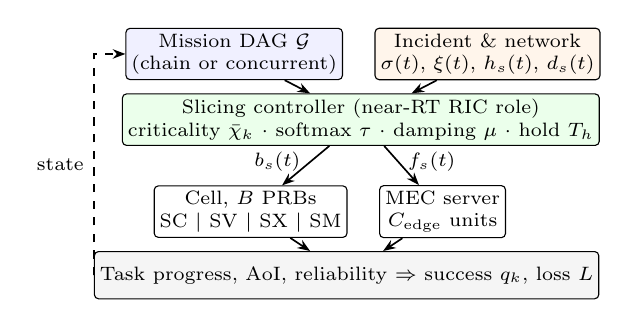
\begin{tikzpicture}[font=\scriptsize, node distance=3mm and 4mm,
  box/.style={draw, rounded corners=1.5pt, align=center, minimum height=6mm, inner sep=2pt},
  arr/.style={-{Stealth[length=1.6mm]}, semithick}]
\node[box, fill=blue!6] (dag) {Mission DAG $\mathcal{G}$\\(chain or concurrent)};
\node[box, fill=orange!8, right=of dag] (env) {Incident \& network\\$\sigma(t)$, $\xi(t)$, $h_s(t)$, $d_s(t)$};
\node[box, fill=green!8, below=5mm of $(dag)!0.5!(env)$, minimum width=50mm] (ctl) {Slicing controller (near-RT RIC role)\\criticality $\bar\chi_k$ $\cdot$ softmax $\tau$ $\cdot$ damping $\mu$ $\cdot$ hold $T_h$};
\node[box, below=5mm of ctl, xshift=-14mm] (gnb) {Cell, $B$ PRBs\\SC $\mid$ SV $\mid$ SX $\mid$ SM};
\node[box, right=of gnb] (mec) {MEC server\\$C_{\mathrm{edge}}$ units};
\node[box, fill=gray!8, below=5mm of $(gnb)!0.5!(mec)$, minimum width=50mm] (out) {Task progress, AoI, reliability $\Rightarrow$ success $q_k$, loss $L$};
\draw[arr] (dag) -- (ctl); \draw[arr] (env) -- (ctl);
\draw[arr] (ctl) -- node[left, pos=0.4]{$b_s(t)$} (gnb);
\draw[arr] (ctl) -- node[right, pos=0.4]{$f_s(t)$} (mec);
\draw[arr] (gnb) -- (out); \draw[arr] (mec) -- (out);
\draw[arr, dashed] (out.west) -- ($(dag.west |- out.west)+(-4mm,0)$) |- node[pos=0.25, left]{state} (dag.west);
\end{tikzpicture}
\caption{MARS-O-RAN digital twin. Each 1\,s step the controller observes mission and network state and allocates PRBs $b_s(t)$, which also set the edge shares $f_s(t)$; the twin then updates task progress, freshness, and reliability.}
\label{fig:system}
\end{figure}

\subsection{Network and Slices}
Time is slotted into steps of $\Delta t=1$\,s over a horizon $T=300$\,s, indexed by integers $t$. The cell has $B$ PRBs ($B=100$ nominally). Let $b_s(t)\in\mathbb{Z}_{\ge0}$ be the PRBs of slice $s\in\mathcal{S}=\{\mathrm{SC},\mathrm{SV},\mathrm{SX},\mathrm{SM}\}$ (robot control, perception video, responder XR, safety sensing). Every allocation must satisfy
\begin{equation}
\sum_{s\in\mathcal{S}} b_s(t)= B,\qquad B_s^{\min}\le b_s(t)\le B_s^{\max},
\label{eq:prb}
\end{equation}
with $B^{\min}=(15,15,10,10)$ and $B^{\max}=(60,60,50,40)$, so $B\ge\sum_s B_s^{\min}=50$ is required. The initial allocation $b(0^-)$ is the equal share $\lfloor B/4\rfloor$ projected onto the bounds, with leftover PRBs assigned in the order SC, SV, SX, SM; at $B=100$ it is 25 PRBs per slice.

\subsection{Mission Task Graph}
The nominal mission is a chain $\mathcal{G}$: $K_1$ gas detection (SV) $\to K_2$ source localization (SM) $\to K_3$ UGV navigation (SC) $\to K_4$ valve inspection (SM) $\to K_5$ valve manipulation (SC). In the \emph{concurrent} variant $\mathcal{G}_c$, the UGV starts approaching the valve area ($K_3$) as soon as the leak is detected, in parallel with localization: $K_1\to\{K_2,K_3\}\to K_4\to K_5$. A task may start once its predecessors have finished and $t\ge t_0$; each slice executes at most one task at a time. A task that overruns its deadline keeps executing until its work is done, and its successors wait for it. Task $k$ has absolute deadline $D_k$, bit workload $L_k$, compute workload $C_k$, value $w_k$, hazard weight $h_k$, freshness limit $\Delta_k^{\max}$, failure budget $\epsilon_k^{\max}$, and slice $s(k)$ (Table~\ref{tab:tasks}).

\begin{table}[t]
\centering
\caption{Mission tasks (synthetic configuration values). $L_k$ in megabits ($10^6$ bits), $C_k$ in compute units (cu); $w_k$, $h_k$, $\epsilon_k^{\max}$ are dimensionless.}
\label{tab:tasks}
\scriptsize
\setlength{\tabcolsep}{2.6pt}
\begin{tabular}{lcrrrrrrr}
\toprule
Task & $s(k)$ & $D_k$ (s) & $L_k$ (Mb) & $C_k$ (cu) & $w_k$ & $h_k$ & $\Delta_k^{\max}$ (s) & $\epsilon_k^{\max}$\\
\midrule
$K_1$ detection & SV & 36 & 0.2 & 20 & 5 & 0.70 & 4 & 0.08\\
$K_2$ localization & SM & 86 & 12.0 & 120 & 8 & 0.80 & 5 & 0.10\\
$K_3$ navigation & SC & 125 & 1.2 & 55 & 10 & 0.95 & 2 & 0.06\\
$K_4$ inspection & SM & 168 & 7.0 & 100 & 9 & 0.90 & 4 & 0.08\\
$K_5$ manipulation & SC & 205 & 1.0 & 50 & 12 & 1.00 & 2 & 0.04\\
\bottomrule
\end{tabular}
\end{table}

\subsection{Incident, Network Shocks, and Demand}
Incident severity is $\sigma(t)=0.05$ for $t<t_0$ and
\begin{equation}
\sigma(t)=\clip\big(\sigma_0+g\,(t-t_0)+n_t,\;0,\;1\big),\quad n_t\sim\mathcal{N}(0,0.025^2),
\label{eq:sev}
\end{equation}
otherwise, with growth $g=0.0015$\,s$^{-1}$ and $\clip(x,a,b)=\max(a,\min(b,x))$. When no shock is active, a 5\,s network shock starts with probability $p_{\mathrm{sh}}(1+\sigma(t))$ per step ($p_{\mathrm{sh}}=0.018$); $\xi(t)\in\{0,1\}$ indicates an active shock. The channel quality of slice $s$ is
\begin{equation}
\begin{aligned}
h_s(t)&=\clip\big(1-\delta(t)+m_{s,t},\;0.45,\;1\big),\\
\delta(t)&=\clip\big(0.15\sigma(t)+0.27\xi(t),\;0,\;0.65\big),
\end{aligned}
\label{eq:chan}
\end{equation}
with $m_{s,t}\sim\mathcal{N}(0,0.018^2)$, and the edge availability is $e(t)=\clip(1-0.25\sigma(t)-0.18\xi(t),\,0.55,\,1)$. Slice demand, in PRB-equivalent units, is
\begin{equation}
d_s(t)=\max\big(8,\;\bar d_s+u_{s,t}+18\,\sigma(t)\,g_s\big),
\label{eq:demand}
\end{equation}
with $u_{s,t}$ drawn from the continuous uniform distribution on $[-7,10]$, $\bar d=(33,27,28,42)$, $g_s=1$ for SV and SM (sensing traffic grows with the hazard) and $g_s=0.4$ otherwise.

\subsection{Radio and Edge Service Model}\label{sec:service}
An executing task $k$ is served by its slice $s=s(k)$. The SNR is $\gamma_s(t)=10^{(\Gamma_s+7\log_{10}h_s(t))/10}$ with nominal SNRs $\Gamma=(18,16,13,12)$\,dB, and the bits delivered in one step are
\begin{equation}
R_s(t)=b_s(t)\,W_{\mathrm{PRB}}\,\log_2\!\big(1+\gamma_s(t)\big)\,\eta\,h_s(t)\,F_s(t)\,\Delta t,
\label{eq:rate}
\end{equation}
with $W_{\mathrm{PRB}}=180$\,kHz, $\eta=0.62$, and $R_s$ in bits ($L_k$ in Table~\ref{tab:tasks} is converted to bits). $F_s$ is a finite-blocklength correction inspired by the normal approximation \cite{polyanskiy},
\begin{equation}
F_s=\clip\!\left(1-\frac{Q^{-1}(\epsilon)\sqrt{V_s/n_s}}{\ln 2\,\log_2(1+\gamma_s)},\,0.55,\,1\right),
\label{eq:fbl}
\end{equation}
with $\epsilon=0.01$ ($Q^{-1}(\epsilon)=2.326$), a simplified dispersion surrogate $V_s=1-1/(1+0.25\gamma_s)$, and $n_s=1800\,b_s$ channel uses (1800 per PRB). Because $b_s\ge10$, $F_s\in[0.994,0.998]$ for every feasible allocation.

The MEC server has $C_{\mathrm{edge}}=100$ compute units shared in proportion to radio share. The MEC scheduler gives every executing task's slice a 15\% priority bonus; this is part of the environment and applies identically to all policies:
\begin{equation}
\begin{aligned}
f_s(t)&=C_{\mathrm{edge}}\,\tilde f_s(t)\Big/\textstyle\sum_{s'}\tilde f_{s'}(t),\\
\tilde f_s(t)&=b_s(t)\big(1+0.15\,\ind{s\in\mathcal{A}(t)}\big),
\end{aligned}
\label{eq:edge}
\end{equation}
where $\mathcal{A}(t)$ is the set of slices with an executing task. Per step, each executing task's remaining work evolves as
\begin{equation}
L_k^{\mathrm{rem}}\leftarrow\big[L_k^{\mathrm{rem}}-R_s(t)\big]^+,\quad C_k^{\mathrm{rem}}\leftarrow\big[C_k^{\mathrm{rem}}-\tfrac{\kappa}{10}f_s(t)\,e(t)\big]^+,
\label{eq:progress}
\end{equation}
with compute efficiency $\kappa=0.72$; the factor $1/10$ converts compute units to work per step. A task finishes at the end of the first step in which both quantities reach zero.

\emph{Compute dominates.} An active slice with 40--60 PRBs delivers about 16--36\,Mb per step, so even $L_2=12$\,Mb clears in under one second, whereas $C_k$ drains at about 2.8--4.0\,cu/s and takes 5--45\,s. Task completion times are therefore set by $f_s(t)$ in \eqref{eq:edge}; PRBs act on outcomes mainly through this coupling and through the load term of the reliability model below.

\subsection{Freshness, Reliability, and Task Success}
AoI of slice $s$ starts at $\Delta_s(0^-)=0$; in each step it resets to 1\,s if $b_s(t)\ge B_s^{\min}+5\cdot\ind{s\in\{\mathrm{SC},\mathrm{SV}\}}$ and grows by 1\,s otherwise, before the completion checks of that step. End-to-end reliability is the product of radio, edge, and backhaul success probabilities,
\begin{equation}
\begin{aligned}
P^{\mathrm{succ}}(t) &= P^{\mathrm{rad}}(t)\,P^{\mathrm{edge}}(t)\,P^{\mathrm{bh}}(t),\\
P^{\mathrm{rad}}(t) &= \big[0.999-0.030\sigma(t)-0.020\,[d_s(t)/b_s(t)-1]^+\\
&\qquad -0.060\xi(t)\big]_{0.82}^{0.999},\\
P^{\mathrm{edge}}(t) &= \big[0.997-0.025\sigma(t)-0.040\xi(t)\big]_{0.84}^{0.997},\\
P^{\mathrm{bh}}(t) &= \big[0.998-0.020\sigma(t)-0.040\xi(t)\big]_{0.85}^{0.998},
\end{aligned}
\label{eq:rel}
\end{equation}
where $[x]_a^b=\clip(x,a,b)$, evaluated at the completion step of the task. Task $k$, finishing at $\tau_k$, succeeds ($q_k=1$) if and only if
\begin{equation}
\tau_k\le D_k,\qquad \Delta_{s(k)}(\tau_k)\le\Delta_k^{\max},\qquad P^{\mathrm{succ}}(\tau_k)\ge 1-\epsilon_k^{\max}.
\label{eq:success}
\end{equation}
A task that does not finish within the horizon counts as failed.

%=====================================================================
\section{Mathematical Problem Formulation}\label{sec:problem}
\subsection{Performance Metrics}
The achieved value of task $k$ is $v_k=w_k$ if $q_k=1$; $v_k=0.45w_k$ if $\tau_k\le D_k$ and $q_k=0$; $v_k=0.10w_k$ if $\tau_k>D_k$; and $v_k=0$ if it never finishes. The \emph{mission loss} is
\begin{equation}
L=\sum_{k\in\mathcal{K}} w_k(1+0.25h_k) - \sum_{k\in\mathcal{K}} v_k,
\label{eq:loss}
\end{equation}
which ranges from $9.875$ (all tasks succeed) to $53.875$ (no task finishes). The \emph{mission-success score} is $\frac{1}{|\mathcal{K}|}\sum_k q_k$; the \emph{full-mission probability} is the fraction of runs in which all five tasks succeed. The reconfiguration cost
\begin{equation}
J_{\mathrm{rc}}=\sum_{t=0}^{T-1}\sum_{s\in\mathcal{S}}\big|b_s(t)-b_s(t-1)\big|
\label{eq:reconfig}
\end{equation}
is a proxy for signalling overhead. Because the mission ends well before $T$, we split it into a mission part over $t\in[t_0,\tau_{\mathrm{end}})$, where $\tau_{\mathrm{end}}$ is the completion of the last task (or $T$), and an idle part over the remaining steps. Tail risk is measured by
\begin{equation}
\mathrm{CVaR}_{\beta}(L)=\min_{\theta\in\mathbb{R}}\Big[\theta+\tfrac{1}{1-\beta}\mathbb{E}\big[(L-\theta)^+\big]\Big],
\label{eq:cvar}
\end{equation}
with $\beta=0.90$ \cite{cvar}. For $N$ runs with losses sorted in decreasing order $L_{(1)}\ge\dots\ge L_{(N)}$ and $m=(1-\beta)N$, we use the exact empirical plug-in
$\widehat{\mathrm{CVaR}}_\beta=\frac{1}{m}\big[\sum_{i=1}^{\lfloor m\rfloor}L_{(i)}+(m-\lfloor m\rfloor)L_{(\lfloor m\rfloor+1)}\big]$,
which averages exactly the worst $m$ runs even when losses are tied.

\subsection{Optimization Problem}
Let $\pi$ be a non-anticipative policy that maps the observed state $x(t)=\{\sigma(t),\xi(t),h(t),e(t),d(t),b(t-1),t_{\mathrm{last}},\text{task states},\Delta(t)\}$ to an allocation $b(t)$, where $t_{\mathrm{last}}$ is the time of the last allocation change. The ideal mission-aware slicing problem is
\begin{equation}
\begin{aligned}
\textbf{(P1)}\quad \min_{\pi}\;\; & \mathbb{E}[L] + \lambda_{\mathrm{cv}}\,\mathrm{CVaR}_{\beta}(L) + \lambda_{\mathrm{rc}}\,\mathbb{E}[J_{\mathrm{rc}}]\\
\text{s.t.}\;\; & \eqref{eq:prb},\; b_s(t)\in\mathbb{Z}_{\ge0}, \quad \forall s,t,\\
& |b_s(t)-b_s(t-1)|\le\Delta_{\max}, \quad \forall s,t,\\
& \text{precedence of }\mathcal{G}\text{ and dynamics }\eqref{eq:sev}\text{--}\eqref{eq:success},
\end{aligned}
\label{eq:p1}
\end{equation}
with $\lambda_{\mathrm{cv}},\lambda_{\mathrm{rc}}\ge0$. (P1) is a finite-horizon stochastic control problem with integer actions, non-convex dynamics, and a tail-risk term; the value of each decision depends on future severity, shocks, and demand, and exact dynamic programming is intractable for a 1\,s loop. We therefore use (P1) in two ways: its objective, with $\lambda_{\mathrm{cv}}=0.5$ and $\lambda_{\mathrm{rc}}=0.001$, is the criterion for tuning MARS (Section~\ref{sec:setup}), and a one-step version of it defines the myopic optimizer baseline.

%=====================================================================
\section{Proposed MARS Controller}\label{sec:mars}
\subsection{Normalized Mission Criticality}
Let $\mathcal{R}(t)$ be the executing tasks together with the tasks that may start at $t$ (in the chain, the executing task or, if none, the next ready task). For $k\in\mathcal{R}(t)$,
\begin{equation}
\chi_k(t)=w_k\big[1+\alpha_u U_k+\alpha_h\,\sigma(t) h_k+\alpha_{cp}I_{cp,k}+\alpha_a A_k\big],
\label{eq:criticality}
\end{equation}
where $U_k=\min\{1,\,40/(\max(D_k-t,0.5)+\varepsilon_u)\}$ is deadline urgency ($\varepsilon_u=2$\,s), $A_k=\min\{3,\Delta_{s(k)}/\max(\Delta_k^{\max},1)\}/3$ is AoI pressure, and $I_{cp,k}$ is the critical-path weight ($1$ for $K_3,K_5$; $0.6$ for $K_2,K_4$; $0.35$ for $K_1$). The hazard and risk coefficients of the earlier version multiplied the same quantity $\sigma h_k$ and are merged into one coefficient $\alpha_h=0.30$. MARS uses the normalized score $\bar\chi_k=\chi_k/\chi_{\mathrm{ref}}\in(0,1]$, with $\chi_{\mathrm{ref}}=\max_k w_k\,(1+\alpha_u+\alpha_h+\alpha_{cp}+\alpha_a)=24$.

\subsection{Slice Weights}
Each slice receives the score
\begin{equation}
\begin{aligned}
u_s(t)={}&\max_{k\in\mathcal{R}(t):\,s(k)=s}\bar\chi_k(t)+\gamma\,\frac{d_s(t)}{\sum_{s'}d_{s'}(t)}\\
&+\ind{\text{mission active}}\,\pi_s\,r(t),
\end{aligned}
\label{eq:score}
\end{equation}
with the maximum taken as 0 if no task maps to $s$, demand weight $\gamma=0.35$, and an optional risk reserve $r(t)=R_0(0.55+0.9\rho)\,g(\sigma,\xi)$, where $g=0.5+\sigma$ during a shock or when $\sigma>0.72$ and $g=\sigma$ otherwise, split as $\pi_{\mathrm{SC}}=0.6$, $\pi_{\mathrm{SV}}=0.4$ (so the split sums to one) and switched off once the mission ends. Weights follow from a temperature-scaled softmax and damping toward the previous allocation,
\begin{equation}
\omega_s=\frac{e^{u_s/\tau}}{\sum_{s'}e^{u_{s'}/\tau}},\qquad \tilde\omega_s=(1-\mu_t)\,\omega_s+\mu_t\,\frac{b_s(t-1)}{B},
\label{eq:softmax}
\end{equation}
and the target is $\hat b_s=\clip(\mathrm{round}(B\tilde\omega_s),B_s^{\min},B_s^{\max})$. The temperature $\tau$ keeps the logits in the unsaturated range of the softmax, so that the criticality values, not only the identity of the active slice, shape the allocation. The damping term $\mu_t\in[0,1)$ pulls the target toward $b(t-1)$ and thus acts directly on the step-to-step change in \eqref{eq:reconfig}.

\subsection{Stability Rules and Task Transitions}
A change of $\mathcal{R}(t)$ starts a \emph{transition}. During a transition, $\mu_t=0$ and no hold is applied, and the transition ends in the step in which the target is reachable within the change limit, i.e., $|\hat b_s-b_s(t-1)|\le\Delta_{\max}$ for all $s$. Outside transitions, $\mu_t=\mu$ and the allocation is held, $b(t)=b(t-1)$, while $t-t_{\mathrm{last}}<T_h^{\mathrm{eff}}(t)$ with the slack-adaptive hold time
\begin{equation}
T_h^{\mathrm{eff}}(t)=T_h\cdot\min\Big\{1,\;\frac{\min_{k\in\mathcal{R}(t)}(D_k-t)^+}{S_{\mathrm{ref}}}\Big\}
\label{eq:hold}
\end{equation}
($T_h^{\mathrm{eff}}=T_h$ when $\mathcal{R}(t)=\emptyset$). Transition mode addresses a flaw of fixed hysteresis: a change limited by $\Delta_{\max}$ would otherwise re-arm the hold and freeze the allocation part-way to its target. Otherwise $\hat b_s$ is clipped to the band $[\max(B_s^{\min},b_s(t-1)-\Delta_{\max}),\min(B_s^{\max},b_s(t-1)+\Delta_{\max})]$. A repair step then enforces $\sum_sb_s=B$ \emph{within the same band}: while the sum exceeds $B$, one PRB is removed from the slice with the largest surplus $b_s-B_s^{\min}$; while it is below $B$, one PRB is added to the slice below its upper band limit with the largest signed unmet demand $d_s-b_s$. Ties, including in $\arg\max$ operations, are broken in the order SC, SV, SX, SM. Because $b(t-1)$ itself satisfies \eqref{eq:prb} and lies in the band, the repair always succeeds, so \eqref{eq:prb} and the change limit hold at every step for every policy. Algorithm~\ref{alg:mars} summarizes one step.

\begin{algorithm}[t]
\caption{One MARS control step at time $t$}
\label{alg:mars}
\small
\begin{algorithmic}[1]
\Require $\sigma(t)$, $\xi(t)$, $d(t)$, $b(t-1)$, $t_{\mathrm{last}}$, $\mathcal{R}(t-1)$, task states
\State $\mathcal{R}\gets$ executing and startable tasks; \textbf{if} $\mathcal{R}\neq\mathcal{R}(t-1)$ \textbf{then} transition $\gets$ true
\State compute $\bar\chi_k$ by \eqref{eq:criticality} and scores $u_s$ by \eqref{eq:score}
\State $\mu_t\gets 0$ if transition else $\mu$;\; $\tilde\omega\gets$ \eqref{eq:softmax}
\State $\hat b_s\gets\clip(\mathrm{round}(B\tilde\omega_s),B_s^{\min},B_s^{\max})$
\If{not transition \textbf{and} $t-t_{\mathrm{last}}<T_h^{\mathrm{eff}}(t)$} \State $b\gets b(t-1)$ \Comment{hold, \eqref{eq:hold}}
\Else
\State \textbf{if} $|\hat b_s-b_s(t-1)|\le\Delta_{\max}\ \forall s$ \textbf{then} transition $\gets$ false
\State $b_s\gets$ $\hat b_s$ clipped to the $\Delta_{\max}$ band
\EndIf
\State repair $\sum_s b_s=B$ within the band
\If{$b\neq b(t-1)$} $t_{\mathrm{last}}\gets t$ \EndIf
\State apply $b$; set edge shares \eqref{eq:edge}; update tasks, AoI, reliability
\end{algorithmic}
\end{algorithm}

\subsection{Complexity}
Scoring costs $O(|\mathcal{K}|+|\mathcal{S}|)$ per step. Because $b(t-1)$ already sums to $B$, the repair moves at most $|\mathcal{S}|\Delta_{\max}$ PRBs, each in $O(|\mathcal{S}|)$, so a step costs $O(|\mathcal{K}|+|\mathcal{S}|^2\Delta_{\max})$. A 300\,s run takes about 30\,ms of Python time on a desktop CPU.

%=====================================================================
\section{Baseline Algorithms and Experimental Setup}\label{sec:setup}
\subsection{Baseline Policies}
All policies use the same environment, including the edge bonus in \eqref{eq:edge}, and the same bounds, change limit, and band-constrained repair.
\begin{itemize}
\item \textbf{STATIC}: fixed shares $(0.29,0.26,0.18,0.27)$, i.e., $b=(29,26,18,27)$ PRBs.
\item \textbf{PROPORTIONAL}: $\omega_s=d_s/\sum_{s'}d_{s'}$.
\item \textbf{MISSION-AWARE}: the unnormalized scores $\chi_k$ in \eqref{eq:score} (without reserve), an 18\% bonus $0.18\max_s u_s$ on the top slice, and a unit-temperature softmax; no damping and no hold. Its logits saturate, so it gives the top-scoring slice its upper bound.
\item \textbf{MYOPIC-OPT}: a one-step version of (P1) with \emph{perfect knowledge of the current state and the service model} but no look-ahead. It enumerates every integer allocation that satisfies \eqref{eq:prb} and the change limit (at most $33^3$ candidates) and minimizes $\sum_{k\in\mathcal{R}}w_k(1+0.25h_k)\big[\hat T_k(b)+50\,\ind{\hat P_k^{\mathrm{succ}}(b)<1-\epsilon_k^{\max}}\big]+\lambda_m\|b-b(t-1)\|_1$, where $\hat T_k=\max\{L_k^{\mathrm{rem}}/R_{s(k)}(b),\,C_k^{\mathrm{rem}}/(\tfrac{\kappa}{10}f_{s(k)}(b)e(t))\}$ is the predicted remaining time, $\lambda_m=0.01$, and SC/SV keep the AoI threshold of 5 PRBs above their minimum when they serve a task. With $\mathcal{R}=\emptyset$ it keeps $b(t-1)$.
\item \textbf{MARS-v0}: the controller of our earlier draft, run in the corrected environment. It uses unnormalized scores, a reserve of $8(0.55+0.9\rho)g(\sigma,\xi)$ PRB-equivalents added with weights 0.45 (SC), 0.35 (SV), and 0.30 (top slice), which sum to 1.10 and accumulate when the top slice is SC or SV, a penalty $0.025|b_s(t-1)-25|$ subtracted from $u_s$, and a fixed 4\,s hold. The penalty depends only on the past allocation, not on the candidate change, and pulls allocations toward 25 PRBs; MARS replaces it with the damping in \eqref{eq:softmax}.
\end{itemize}
MISSION-AWARE and MARS differ in several mechanisms at once (bonus, normalization, temperature, damping, hold, transition mode); the ablation in Section~\ref{sec:ablation} isolates each of them.

\subsection{Operating Points, Seeds, and Parameters}
We evaluate three operating points: \textbf{OP-A}, the chain mission at $\sigma_0=0.2$, where all tasks are feasible; \textbf{OP-B}, the chain mission at $\sigma_0=0.6$, a severe incident in which $K_5$ is infeasible for every policy (Section~\ref{sec:k5}); and \textbf{OP-C}, the concurrent mission $\mathcal{G}_c$ at $\sigma_0=0.2$. Each policy runs for 300\,s on evaluation seeds 20--319 (300 seeds, 5400 runs). Every random draw (severity noise, shocks, channel, demand) is consumed in the same order regardless of the policy, so a seed gives all policies an identical environment trajectory; we verify this programmatically and use paired tests. All data are synthetic and generated by the simulator. Table~\ref{tab:params} lists the parameters.

\begin{table}[t]
\centering
\caption{Simulation and controller parameters.}
\label{tab:params}
\scriptsize
\setlength{\tabcolsep}{2.5pt}
\begin{tabular}{lll}
\toprule
Group & Parameter & Value\\
\midrule
Simulation & horizon $T$, step $\Delta t$ & 300\,s, 1\,s\\
 & seeds: eval.\ / sweeps / tuning & 20--319 / 20--119 / 1000--1099\\
Radio & $B$, $W_{\mathrm{PRB}}$, $\eta$ & 100 PRBs, 180\,kHz, 0.62\\
 & channel uses per PRB & 1800\\
 & $B^{\min}$, $B^{\max}$ (SC,SV,SX,SM) & (15,15,10,10), (60,60,50,40)\\
 & nominal SNR $\Gamma_s$ & (18,16,13,12)\,dB\\
Edge & $C_{\mathrm{edge}}$, $\kappa$, task bonus & 100\,cu, 0.72, 15\% (all)\\
Incident & $t_0$, $\sigma_0$ (OP-A/C, OP-B), $g$ & 20\,s, 0.2 / 0.6, 0.0015\,s$^{-1}$\\
 & $p_{\mathrm{sh}}$, shock duration & 0.018/step, 5\,s\\
Demand & $\bar d$ (SC,SV,SX,SM), $u_{s,t}$ & (33,27,28,42), $\mathcal{U}[-7,10]$\\
Criticality & $\alpha_u,\alpha_h,\alpha_{cp},\alpha_a$ & 0.40, 0.30, 0.20, 0.10\\
 & $\varepsilon_u$, demand weight $\gamma$ & 2\,s, 0.35\\
MARS & $\tau$, $\mu$, $T_h$, $S_{\mathrm{ref}}$, $R_0$ & 0.8, 0.25, 8\,s, 10\,s, 0 (tuned)\\
All & change limit $\Delta_{\max}$, risk aversion $\rho$ & 16 PRBs/step, 0.55\\
MARS-v0 & reserve, penalty, hold & 8 PRB-eq., 0.025, 4\,s\\
MYOPIC-OPT & $\lambda_m$ & 0.01\\
Metrics & CVaR level $\beta$; bootstrap & 0.90; 4000 resamples (seed 7)\\
\bottomrule
\end{tabular}
\end{table}

\subsection{Tuning Protocol}
The five MARS parameters were selected by grid search on the disjoint tuning seeds 1000--1099, minimizing the (P1) objective $\mathbb{E}[L]+0.5\,\mathrm{CVaR}_{0.9}(L)+0.001\,\mathbb{E}[J_{\mathrm{rc}}]$ averaged over the three operating points. The grid was $\tau\in\{0.1,0.2,0.4,0.8,1.2,1.6\}$, $R_0\in\{0,0.2\}$, $\mu\in\{0.25,0.5,0.75,0.9\}$, $T_h\in\{4,8,12,20\}$\,s, and $S_{\mathrm{ref}}\in\{10,20,40\}$\,s (576 configurations). The selected $\tau$ and $T_h$ are interior to the grid (values of $\tau$ above 0.8 were clearly worse), whereas $\mu=0.25$, $S_{\mathrm{ref}}=10$\,s, and $R_0=0$ lie at the lower edge; the sweeps in \figref{fig:params} extend to $\mu=0$ without improvement. In particular, the search \emph{switches the risk reserve off}, because the reserve never lowered the objective. Baseline parameters were not tuned.

\subsection{Statistical Analysis}
We report 95\% percentile bootstrap confidence intervals (4000 resamples) for means and CVaR \cite{bootstrap}. Paired comparisons use per-seed differences and Wilcoxon signed-rank tests \cite{wilcoxon}; zero differences are discarded, so we also report the number of non-tied pairs $N_{\mathrm{eff}}$. With 300 seeds, CVaR$_{0.90}$ averages the worst 30 runs.

\subsection{Edge-Case Studies}
Table~\ref{tab:edge} lists the sweeps around OP-A, each with all six policies (or MARS alone for its parameters, at all three operating points) on seeds 20--119. Deadline scaling stretches each deadline relative to the incident start, $D_k'=t_0+s(D_k-t_0)$, rounded to the nearest second; workload scaling multiplies both $L_k$ and $C_k$.

\begin{table}[t]
\centering
\caption{Edge-case studies (100 seeds per point).}
\label{tab:edge}
\scriptsize
\begin{tabular}{lll}
\toprule
Study & Values & Edge case probed\\
\midrule
PRB budget $B$, fixed caps & 50--200 & feasibility floor; surplus\\
PRB budget $B$, caps $\propto B$ & 50--200 & radio--edge coupling\\
Initial severity $\sigma_0$ & 0--1.0 & benign vs.\ extreme incident\\
Shock prob.\ $p_{\mathrm{sh}}$ & 0--0.30 & no shocks vs.\ shock storm\\
Deadline scale & 0.5--1.5 & infeasible vs.\ relaxed deadlines\\
Workload scale & 0.25--3.0 & light load vs.\ horizon overrun\\
Severity $\times$ $B$ grid & $5\times4$ & joint stress\\
MARS $\tau,R_0,\mu,T_h,\Delta_{\max}$ & see \figref{fig:params} & controller sensitivity\\
Ablation (15 variants, 300 seeds) & --- & component contribution\\
\bottomrule
\end{tabular}
\end{table}

%=====================================================================
\section{Results at the Three Operating Points}\label{sec:results}
\subsection{Aggregate Performance}
Table~\ref{tab:main} and \figref{fig:ci} report the main results. Mission awareness is decisive: at OP-A the success score rises from 0.361 (STATIC) and 0.713 (PROPORTIONAL) to 0.906--0.924 for the four mission-oriented controllers, which are the only ones that ever complete the full mission. At OP-B, STATIC and PROPORTIONAL miss the deadline of $K_2$ and every later deadline (80\% of their task instances fail on deadlines), and their success falls to 0.181. The four mission-oriented controllers have overlapping confidence intervals for success, loss, and CVaR at OP-A and OP-C. They differ sharply in reconfiguration: during the mission MARS changes 216 PRB-steps at OP-A, against 1354 for MISSION-AWARE, 575 for MARS-v0, and 310 for the optimizer. In the idle windows MISSION-AWARE and MARS-v0 keep reconfiguring (407 and 498 PRB-steps) in response to demand noise and, for MARS-v0, a reserve that stays on after the mission; MARS changes 82 and MYOPIC-OPT none.

\begin{table*}[t]
\centering
\caption{Main results, 300 paired seeds per policy: mean [95\% bootstrap CI]. Reconfiguration is split into the mission window $[t_0,\tau_{\mathrm{end}})$ and the idle remainder.}
\label{tab:main}
\footnotesize
\setlength{\tabcolsep}{4pt}
\begin{tabular}{lcccccc}
\toprule
Policy & Success score & Full-mission prob. & Mean loss $L$ & CVaR$_{0.90}(L)$ & $J_{\mathrm{rc}}$ mission & $J_{\mathrm{rc}}$ idle\\
\midrule
\multicolumn{7}{l}{\emph{OP-A: benign ($\sigma_0=0.2$), chain mission}}\\
STATIC & 0.361 [0.351, 0.370] & 0.000 & 32.59 [32.37, 32.82] & 37.46 [36.82, 37.73] & 0 & 14\\
PROPORTIONAL & 0.713 [0.699, 0.726] & 0.000 & 18.74 [18.37, 19.12] & 26.02 [24.78, 27.27] & 2233 & 1589\\
MISSION-AWARE & 0.906 [0.891, 0.921] & 0.603 & 12.27 [11.89, 12.65] & 19.02 [17.83, 20.40] & 1354 & 407\\
MYOPIC-OPT & 0.906 [0.891, 0.920] & 0.603 & 12.27 [11.90, 12.65] & 18.91 [17.80, 20.18] & 310 & 0\\
MARS-v0 & 0.924 [0.909, 0.939] & 0.687 & 11.78 [11.41, 12.15] & 18.75 [17.45, 20.11] & 575 & 498\\
\textbf{MARS} & 0.909 [0.894, 0.923] & 0.627 & 12.08 [11.74, 12.44] & 18.97 [17.78, 20.01] & 216 & 82\\
\midrule
\multicolumn{7}{l}{\emph{OP-B: severe ($\sigma_0=0.6$), chain mission}}\\
STATIC & 0.181 [0.175, 0.188] & 0.000 & 45.23 [45.14, 45.32] & 47.54 [46.62, 47.72] & 0 & 14\\
PROPORTIONAL & 0.181 [0.175, 0.187] & 0.000 & 45.21 [45.12, 45.31] & 47.54 [46.72, 47.72] & 2246 & 1174\\
MISSION-AWARE & 0.696 [0.681, 0.711] & 0.000 & 18.94 [18.58, 19.29] & 25.81 [24.36, 27.00] & 1496 & 348\\
MYOPIC-OPT & 0.695 [0.681, 0.710] & 0.000 & 18.95 [18.59, 19.30] & 25.50 [24.12, 26.85] & 310 & 0\\
MARS-v0 & 0.692 [0.677, 0.707] & 0.000 & 19.09 [18.73, 19.45] & 25.88 [24.47, 26.83] & 615 & 326\\
\textbf{MARS} & 0.667 [0.651, 0.683] & 0.000 & 19.58 [19.20, 19.96] & 26.25 [25.35, 26.89] & 242 & 83\\
\midrule
\multicolumn{7}{l}{\emph{OP-C: benign ($\sigma_0=0.2$), concurrent mission ($K_2\parallel K_3$)}}\\
STATIC & 0.585 [0.569, 0.600] & 0.000 & 23.59 [23.19, 23.99] & 29.95 [29.18, 30.84] & 0 & 14\\
PROPORTIONAL & 0.687 [0.670, 0.703] & 0.003 & 19.69 [19.23, 20.18] & 28.93 [26.98, 30.39] & 1833 & 1990\\
MISSION-AWARE & 0.910 [0.895, 0.924] & 0.627 & 12.13 [11.78, 12.50] & 19.01 [17.92, 20.18] & 1246 & 418\\
MYOPIC-OPT & 0.912 [0.898, 0.925] & 0.620 & 12.07 [11.74, 12.43] & 18.53 [17.56, 19.61] & 252 & 0\\
MARS-v0 & 0.915 [0.901, 0.929] & 0.640 & 12.03 [11.67, 12.40] & 19.04 [17.89, 20.27] & 515 & 520\\
\textbf{MARS} & 0.916 [0.903, 0.930] & 0.650 & 12.00 [11.63, 12.35] & 18.69 [17.69, 19.87] & 158 & 83\\
\bottomrule
\end{tabular}

\end{table*}

\begin{figure*}[!tp]
\centering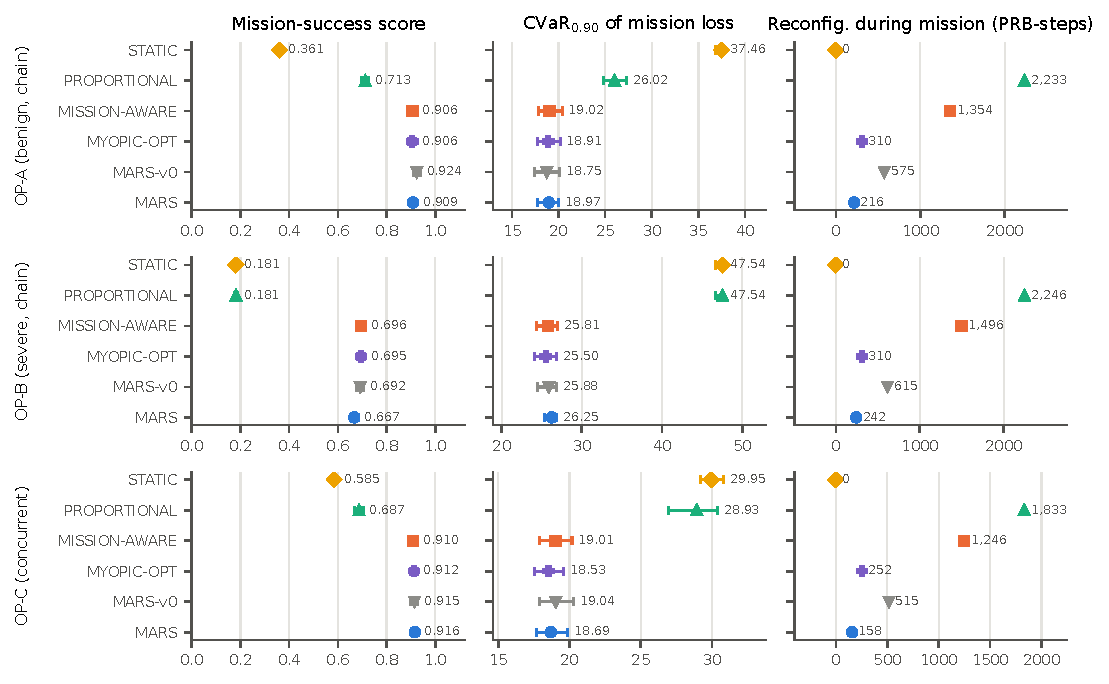
\includegraphics[width=\textwidth]{fig_main_ci.pdf}
\caption{Main metrics with 95\% bootstrap confidence intervals (300 seeds) at the three operating points. STATIC never reconfigures during the mission; its only change is the move from the equal-share initial allocation.}
\label{fig:ci}
\end{figure*}

\subsection{Paired Comparisons}
Table~\ref{tab:paired} compares MARS seed by seed with the three strongest baselines. At OP-A and OP-C, none of the differences in success or loss is significant ($p\ge0.08$), and most pairs are tied (e.g., 155 of 300 against MISSION-AWARE at OP-A). MARS reconfigures less during the mission than every baseline in all 300 seeds: by 84.0\% and 87.3\% relative to MISSION-AWARE, 30.2\% and 37.5\% relative to MYOPIC-OPT, and 62.3\% and 69.4\% relative to MARS-v0 at OP-A and OP-C. At OP-B the stability mechanisms have a measurable cost: MARS loses 0.029 in success against MISSION-AWARE ($p=0.015$) and 0.64 in mean loss ($p=0.005$). \figref{fig:pareto} shows the resulting trade-off per run.

\begin{table*}[t]
\centering
\caption{Paired differences MARS $-$ baseline over 300 seeds. Success: mean [95\% CI], win/tie/loss count for MARS, number of non-tied pairs $N_{\mathrm{eff}}$, and Wilcoxon $p$. Loss: mean difference and $p$. Last column: relative change of reconfiguration during the mission (MARS lower in all 300 seeds for every row).}
\label{tab:paired}
\footnotesize
\begin{tabular}{llccccccc}
\toprule
OP & Baseline & $\Delta$ success [CI] & W/T/L & $N_{\mathrm{eff}}$ & $p$ & $\Delta$ loss & $p$ & $\Delta J_{\mathrm{rc}}$ mission\\
\midrule
OP-A & MISSION-AWARE & $+0.003$ [$-0.017, +0.021$] & 75/155/70 & 145 & 0.939 & $-0.19$ & 0.355 & $-84.0\%$\\
 & MYOPIC-OPT & $+0.003$ [$-0.016, +0.021$] & 76/154/70 & 146 & 0.989 & $-0.19$ & 0.323 & $-30.2\%$\\
 & MARS-v0 & $-0.015$ [$-0.032, +0.001$] & 50/184/66 & 116 & 0.081 & $+0.30$ & 0.213 & $-62.3\%$\\
\midrule
OP-B & MISSION-AWARE & $-0.029$ [$-0.051, -0.007$] & 74/115/111 & 185 & 0.015 & $+0.64$ & 0.005 & $-83.8\%$\\
 & MYOPIC-OPT & $-0.028$ [$-0.049, -0.007$] & 76/114/110 & 186 & 0.015 & $+0.63$ & 0.005 & $-21.9\%$\\
 & MARS-v0 & $-0.025$ [$-0.044, -0.005$] & 55/151/94 & 149 & 0.026 & $+0.49$ & 0.055 & $-60.6\%$\\
\midrule
OP-C & MISSION-AWARE & $+0.006$ [$-0.009, +0.022$] & 54/198/48 & 102 & 0.534 & $-0.14$ & 0.668 & $-87.3\%$\\
 & MYOPIC-OPT & $+0.004$ [$-0.015, +0.024$] & 70/168/62 & 132 & 0.807 & $-0.08$ & 0.732 & $-37.5\%$\\
 & MARS-v0 & $+0.001$ [$-0.017, +0.021$] & 70/164/66 & 136 & 0.837 & $-0.03$ & 0.913 & $-69.4\%$\\
\bottomrule
\end{tabular}

\end{table*}

\begin{figure*}[!tp]
\centering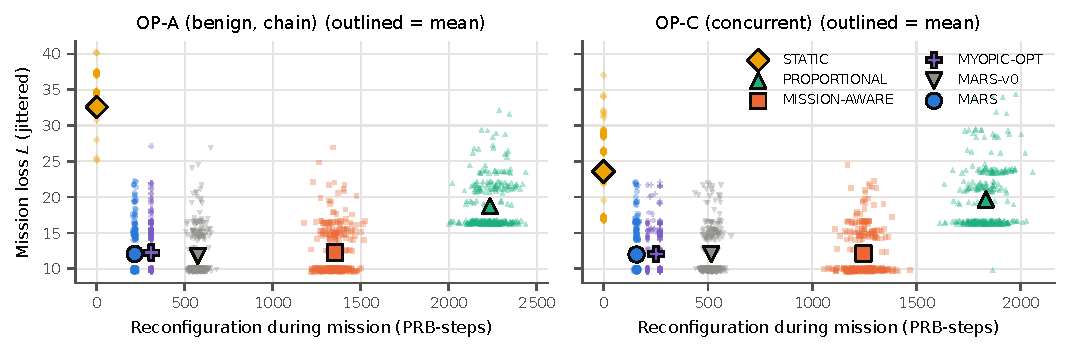
\includegraphics[width=\textwidth]{fig_pareto.pdf}
\caption{Per-run mission loss versus reconfiguration during the mission (jitter $\pm0.3$ on loss; outlined markers are means). The mission-oriented controllers reach the same loss; MARS reaches it with the fewest changes.}
\label{fig:pareto}
\end{figure*}

\subsection{Tail Risk}
\figref{fig:cvar} plots CVaR$_\beta$ for $\beta\in[0,0.95]$ with the exact estimator. The mission-oriented controllers have nearly identical tail curves at every operating point, and at $\beta=0.90$ their CVaR intervals overlap (Table~\ref{tab:main}). An earlier version of this study used the mean of losses at or above the $\beta$-quantile; with tied losses that estimator averaged more than the worst $(1-\beta)N$ runs and produced an apparent CVaR advantage for MARS-v0 (23.26 vs.\ 24.54 for MISSION-AWARE over 30 seeds). The exact estimator gives 24.54 for both, so the advantage was an estimator artifact. No controller has a tail-risk advantage in this model.

\begin{figure*}[!tp]
\centering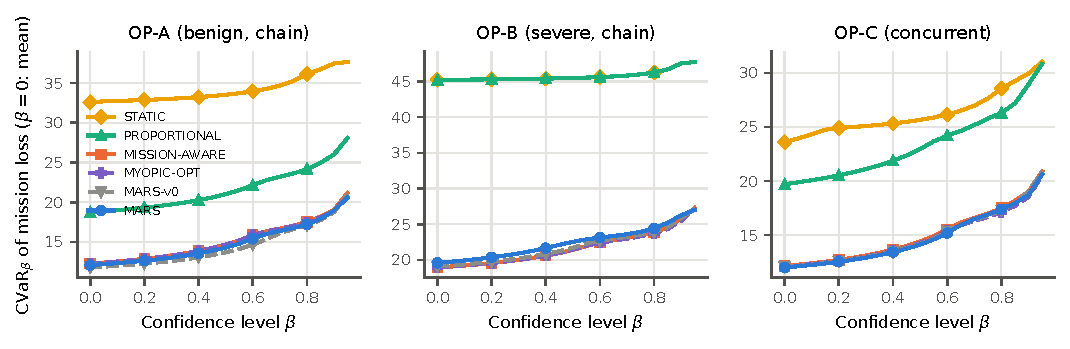
\includegraphics[width=\textwidth]{fig_cvar_beta.pdf}
\caption{CVaR$_\beta$ of mission loss versus $\beta$ (exact estimator, 300 seeds; $\beta=0$ is the mean).}
\label{fig:cvar}
\end{figure*}

\subsection{Per-Task Anatomy}\label{sec:k5}
\figref{fig:tasks} breaks success down by task and \figref{fig:attr} attributes every failure at OP-A to its first failed check. The mission-oriented controllers meet every deadline at all three operating points; their failures are reliability failures. AoI is not binding: of 27{,}000 task instances, 6 failed the freshness check, all under PROPORTIONAL.

$K_5$ never succeeds at OP-B. It requires $P^{\mathrm{succ}}\ge0.96$, and ignoring load and shock terms \eqref{eq:rel} gives $P^{\mathrm{succ}}=(0.999-0.030\sigma)(0.997-0.025\sigma)(0.998-0.020\sigma)$, which falls below 0.96 for $\sigma>0.46$; at OP-B severity exceeds this from $t_0$ on. This is why OP-A, where $K_5$ succeeds in 88--94\% of runs for the mission-oriented controllers, is our primary operating point.

MARS succeeds less often on $K_3$ at OP-B (0.690 vs.\ 0.800 for MISSION-AWARE). Extra PRBs on SC do not help reliability once $b_{\mathrm{SC}}\ge d_{\mathrm{SC}}$, because the load term in \eqref{eq:rel} vanishes; what matters is when $K_3$ finishes. Under MARS, $K_3$ finishes on average at 98.4\,s instead of 90.5\,s, because the softer softmax gives the active slice fewer PRBs and thus a smaller edge share. Severity at completion is then higher (0.717 vs.\ 0.703), close to the $K_3$ reliability threshold ($\sigma\approx0.74$ without load and shock terms), so a shock during completion more often causes failure.

\begin{figure*}[!tp]
\centering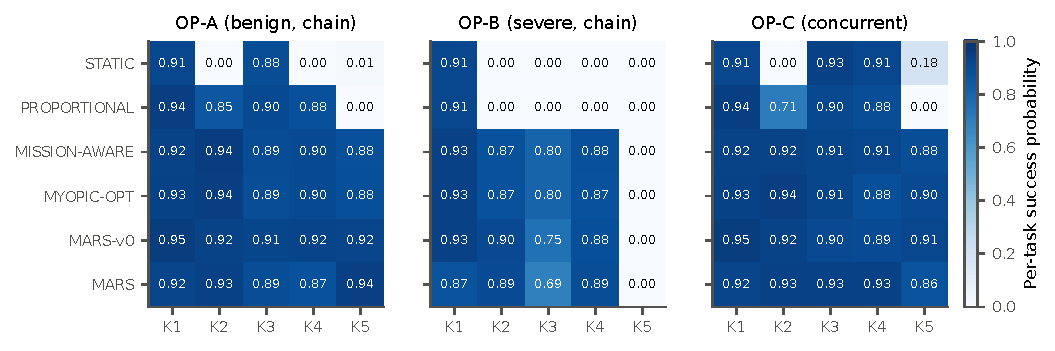
\includegraphics[width=\textwidth]{fig_task_success.pdf}
\caption{Per-task success probability (300 seeds). $K_5$ is infeasible at OP-B for every policy.}
\label{fig:tasks}
\end{figure*}

\begin{figure}[t]
\centering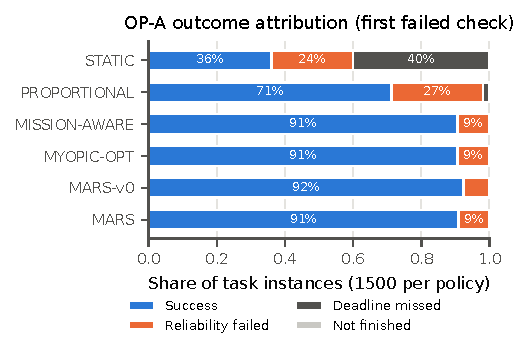
\includegraphics[width=\columnwidth]{fig_attribution.pdf}
\caption{OP-A: outcome of all 1500 task instances per policy, attributed to the first failed check (deadline, then reliability or freshness); tasks unfinished at the horizon are shown separately.}
\label{fig:attr}
\end{figure}

\subsection{Allocation Dynamics and Criticality}
\figref{fig:gantt} shows the task timeline for seed 20 at OP-A; the mission ends at 133\,s under MISSION-AWARE and MYOPIC-OPT, at 140\,s under MARS-v0, and at 144\,s under MARS. Averaged over 300 seeds, MARS completes the mission 10.7\,s later than MISSION-AWARE (143.8 vs.\ 133.1\,s), still well inside all deadlines.

\figref{fig:trace} shows the concurrent mission (OP-C), the setting in which criticality can matter. In MARS-v0 the largest softmax weight averages 0.996 during the mission, so the controller allocates by slice identity alone. In MARS it averages 0.395, so allocations depend on the criticality values. While $K_2$ (SM) and $K_3$ (SC) run in parallel, MISSION-AWARE gives 57 PRBs to SC and 15 to SM on average (100 seeds), starving localization; MARS gives 35 and 32, close to the 34 and 39 chosen by the model-based optimizer. After the mission, MARS keeps a nearly constant allocation, whereas MISSION-AWARE follows demand noise and MARS-v0 follows its reserve. The control-latency proxy $8+0.55[35-b_{\mathrm{SC}}]^++7\sigma+8\xi+\mathcal{U}[0,2.5]$\,ms, a diagnostic that does not enter task success, averages 16.9--17.8\,ms during the mission for all four mission-oriented controllers at OP-A. After the mission it is 19.3 and 19.2\,ms for MARS and MISSION-AWARE and 13.7--14.3\,ms for MYOPIC-OPT and MARS-v0, which keep more PRBs on SC; these differences arise outside the mission and do not reflect better mission service.

\begin{figure*}[!tp]
\centering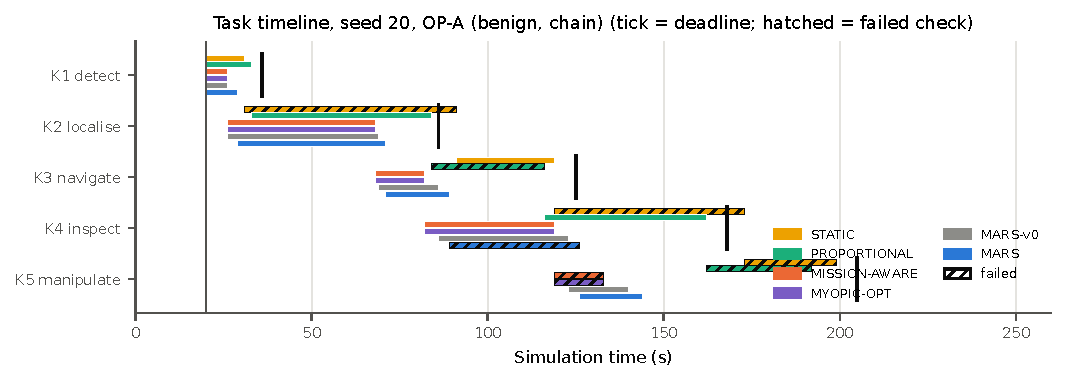
\includegraphics[width=\textwidth]{fig_gantt_seed20.pdf}
\caption{Task timeline for seed 20 at OP-A. All mission-oriented controllers meet every deadline; MARS finishes later because it serves the active slice with fewer PRBs.}
\label{fig:gantt}
\end{figure*}

\begin{figure*}[!tp]
\centering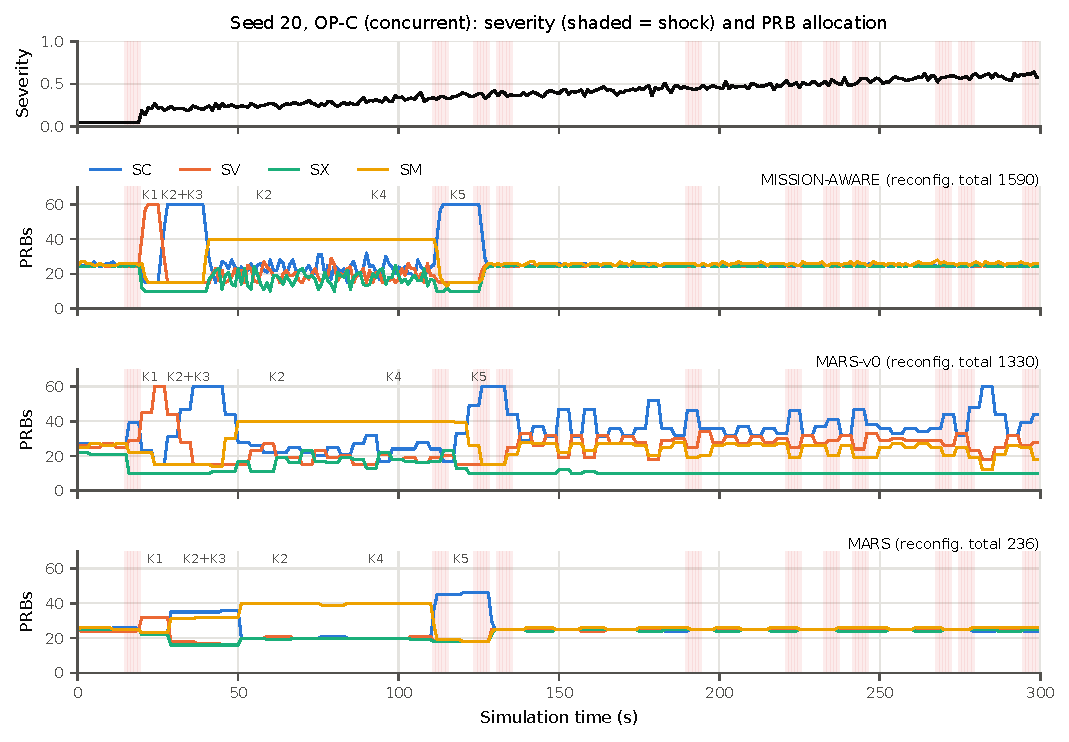
\includegraphics[width=\textwidth]{fig_trace_C_concurrent.pdf}
\caption{Seed 20, concurrent mission (OP-C): severity with shocks (shaded) and PRB allocations. During $K_2\parallel K_3$, MISSION-AWARE saturates SC while MARS splits the cell between SC and SM; MARS's allocation is piecewise constant and almost flat after the mission.}
\label{fig:trace}
\end{figure*}

%=====================================================================
\section{Edge-Case Evaluation}\label{sec:edge}
\subsection{Radio Budget and Radio--Edge Coupling}
\figref{fig:prb} sweeps $B$. At $B=50=\sum_sB_s^{\min}$ every slice is pinned at its minimum and all success scores are zero; smaller budgets violate \eqref{eq:prb} and are rejected by the configuration validator. With fixed slice caps (\figref{fig:prb}(a)), success falls for $B>120$ and reaches the STATIC level at $B=200$ (0.19 for every policy). The cause is the coupling in \eqref{eq:edge}: the active SM slice is capped at 40 PRBs, so its edge share is $46/(B+6)$, which drops from 43\% at $B=100$ to 29\% at $B=150$ and makes $K_2$ miss its deadline. When the caps scale with $B$ (\figref{fig:prb}(b)), the paradox disappears: MISSION-AWARE reaches 0.932 and MARS 0.916 at $B=200$. The paradox is thus an artifact of tying edge shares to radio shares under fixed caps, the situation that joint radio--edge slicing \cite{sledge,elbamby} avoids. MARS is weak when PRBs are scarce: at $B=55$ and $B=60$ it reaches 0.146 and 0.538, against 0.440 and 0.754 for MISSION-AWARE, because its unsaturated softmax spends PRBs on slices without tasks.

\begin{figure*}[!tp]
\centering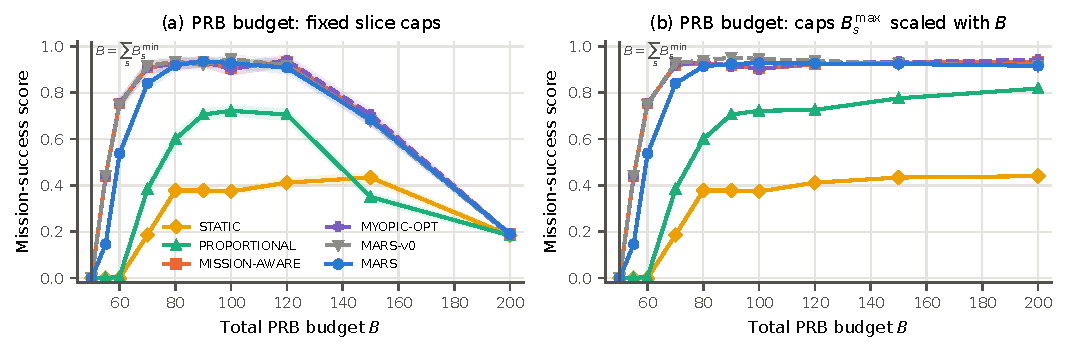
\includegraphics[width=\textwidth]{fig_sweep_prbs.pdf}
\caption{PRB-budget sweep (100 seeds; shaded bands in (a) are 95\% CIs). (a) Fixed slice caps; the vertical line marks $B=\sum_sB_s^{\min}=50$. (b) Caps $B_s^{\max}$ scaled with $B$: the decline above $B=120$ disappears.}
\label{fig:prb}
\end{figure*}

\subsection{Incident Severity and Network Shocks}
\figref{fig:sev} varies $\sigma_0$. Under a benign incident MARS performs best on the tail: at $\sigma_0=0$ its success is 0.940 [0.920, 0.958] against 0.922 [0.896, 0.946] for MISSION-AWARE, with CVaR$_{0.90}$ 16.92 vs.\ 19.83. As severity grows, all policies degrade, and at extreme severity MARS degrades most: at $\sigma_0=1.0$ it reaches 0.152 against 0.368 for MISSION-AWARE. \figref{fig:shock} sweeps the shock probability. Without shocks all mission-oriented controllers succeed in every task (1.000). Under frequent shocks MARS and MARS-v0 hold up slightly better than MISSION-AWARE and MYOPIC-OPT (0.708 and 0.710 vs.\ 0.678 and 0.672 at $p_{\mathrm{sh}}=0.08$), and all reach 0.24--0.28 in a shock storm ($p_{\mathrm{sh}}=0.3$).

\begin{figure*}[!tp]
\centering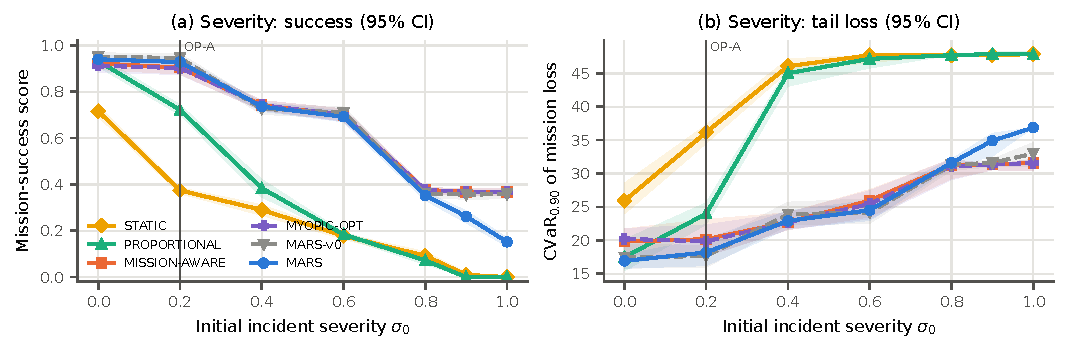
\includegraphics[width=\textwidth]{fig_sweep_severity.pdf}
\caption{Initial-severity sweep (100 seeds, 95\% CIs). The vertical line marks OP-A.}
\label{fig:sev}
\end{figure*}

\begin{figure*}[!tp]
\centering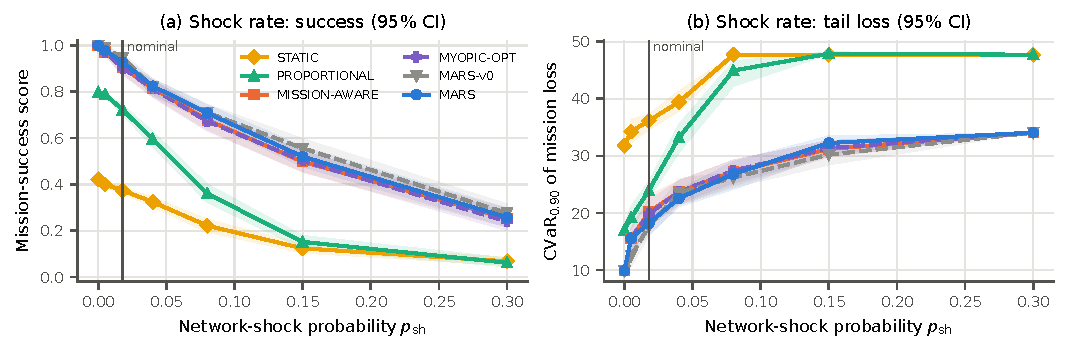
\includegraphics[width=\textwidth]{fig_sweep_shock.pdf}
\caption{Network-shock probability sweep (100 seeds, 95\% CIs; vertical line = nominal $p_{\mathrm{sh}}=0.018$).}
\label{fig:shock}
\end{figure*}

\subsection{Deadline Tightness and Workload}
Tight deadlines and heavy workloads expose the same weakness as scarce PRBs (\figref{fig:deadline}, \figref{fig:workload}). At deadline scale 0.7, MARS reaches 0.558 against 0.712 for MISSION-AWARE and MYOPIC-OPT; at 0.5 it completes no task successfully, while the others still complete $K_1$. At $1.5\times$ workload MARS reaches 0.356 against 0.626 for MISSION-AWARE, and at $2\times$ and $3\times$ it scores zero while the other mission-oriented controllers reach 0.15--0.19. In each case the active task needs every PRB its slice can get, and MARS's softer allocation delays it past a deadline. Relaxed deadlines (scale 1.5) help STATIC and PROPORTIONAL most (0.732 and 0.730), since deadlines were their binding constraint; at light load ($0.25\times$) all policies reach 0.91--0.93.

\begin{figure*}[!tp]
\centering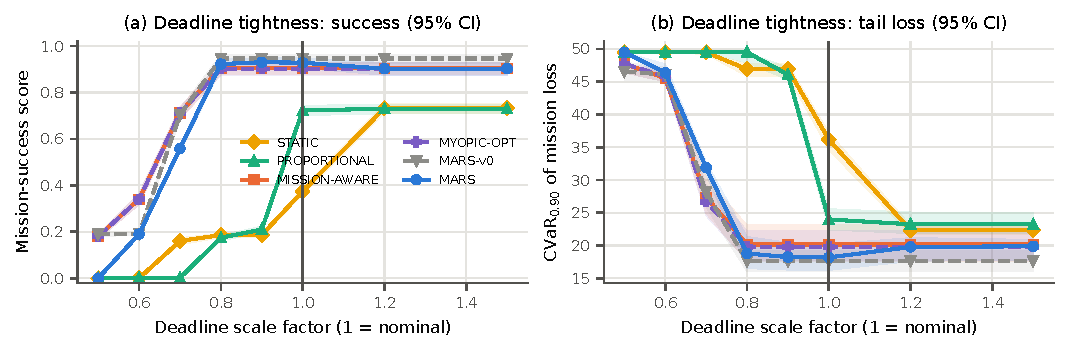
\includegraphics[width=\textwidth]{fig_sweep_deadline.pdf}
\caption{Deadline-scale sweep (100 seeds). Below scale 0.8 MARS trails MISSION-AWARE and MYOPIC-OPT.}
\label{fig:deadline}
\end{figure*}

\begin{figure*}[!tp]
\centering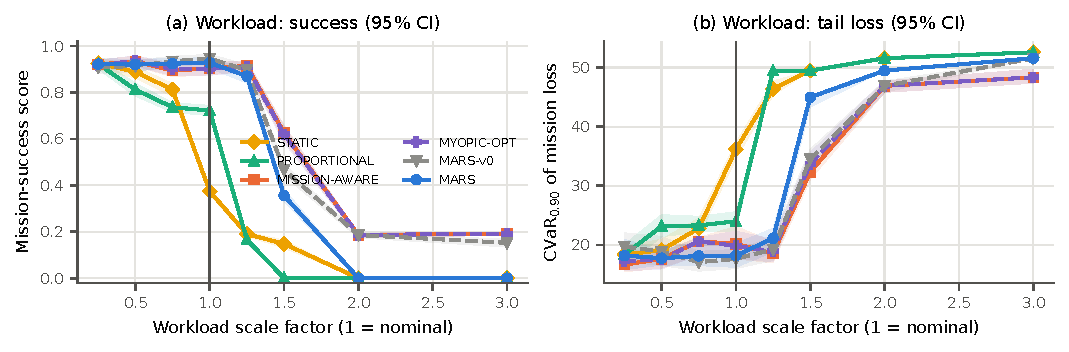
\includegraphics[width=\textwidth]{fig_sweep_workload.pdf}
\caption{Workload-scale sweep (100 seeds). Above $1.25\times$ success drops for every policy, and fastest for MARS.}
\label{fig:workload}
\end{figure*}

\subsection{Joint Stress}
Across the $5\times4$ grid of $\sigma_0\in\{0.2,\dots,1.0\}$ and $B\in\{60,80,100,120\}$, MARS is within 0.03 of MISSION-AWARE in 9 of 20 cells and behind by more in the other 11, by up to 0.45 at $\sigma_0=0.4$, $B=60$; the largest deficits are at $B=60$ and at $\sigma_0=1.0$ (full table in the released results).

\subsection{MARS Parameters and Ablation}\label{sec:ablation}
\figref{fig:params} sweeps the MARS parameters at all three operating points. The temperature $\tau$ is the main lever: from $\tau=0.05$ to $0.8$, reconfiguration during the mission falls from 516 to 216 PRB-steps at OP-A with unchanged success, and at $\tau=1.6$ success collapses (0.312 at OP-B). The hold time and damping further reduce reconfiguration with almost no effect on success. A positive reserve scale $R_0$ does not improve success and, at $R_0=0.8$, lowers it at OP-B (0.562). A change limit $\Delta_{\max}\le8$ slows transitions and costs success at OP-B.

The ablation (\figref{fig:ablation}, 300 seeds) isolates each mechanism.
(i) Without the transition mode (fixed hold, no slack adaptation) success drops to 0.887 at OP-A and 0.635 at OP-B, the largest loss of any variant; transition mode is what keeps MARS agile.
(ii) A saturated softmax ($\tau=0.05$) raises reconfiguration to 515 PRB-steps at OP-A, and removing the hold time raises it to 307; removing damping alone changes little (226).
(iii) Removing all criticality terms leaves success unchanged (0.920 vs.\ 0.909 at OP-A, 0.921 vs.\ 0.916 at OP-C) but raises reconfiguration by 24--44\%. With normalization, criticality now shapes the allocation, as \figref{fig:trace} shows, but in this model it buys stability, not mission success.
(iv) For MARS-v0, removing both the reserve and the penalty leaves success and reconfiguration essentially unchanged (0.912 vs.\ 0.924 and 571 vs.\ 575 PRB-steps at OP-A); its savings over MISSION-AWARE came entirely from the hold time.
(v) Removing the edge bonus changes the success of MARS and MISSION-AWARE by at most 0.011 at OP-A, so the bonus does not drive the comparison once it applies to all policies.

\begin{figure*}[!tp]
\centering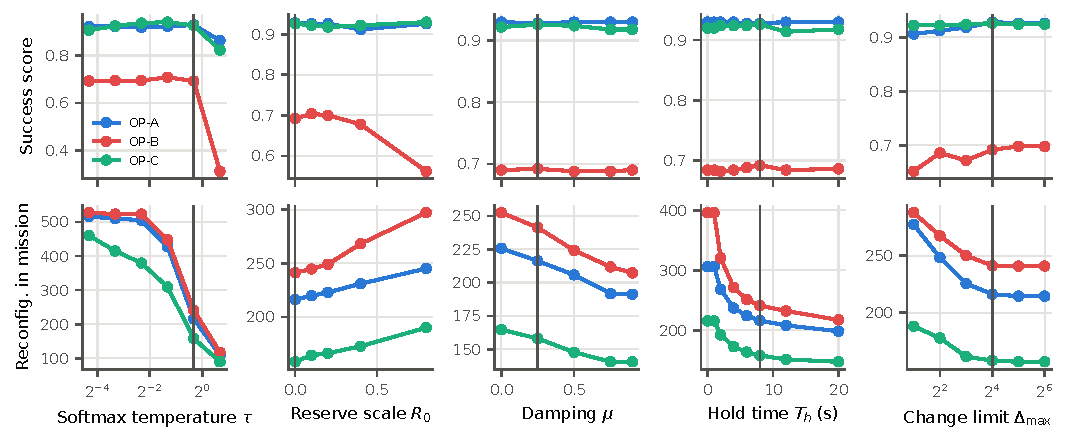
\includegraphics[width=\textwidth]{fig_mars_params.pdf}
\caption{MARS parameter sensitivity at the three operating points (100 seeds; vertical lines mark the tuned values). Top: success score. Bottom: reconfiguration during the mission.}
\label{fig:params}
\end{figure*}

\begin{figure*}[!tp]
\centering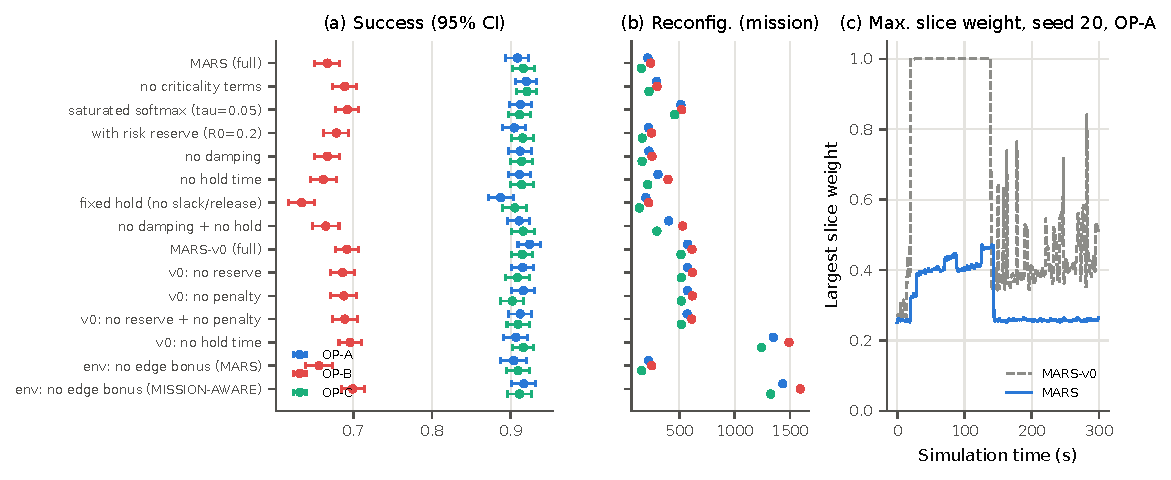
\includegraphics[width=\textwidth]{fig_ablation.pdf}
\caption{(a,b) Ablation over 300 seeds (95\% CIs) at the three operating points. (c) Largest slice weight per step on seed 20 at OP-A: MARS-v0 is saturated at 1 during the mission, MARS is not.}
\label{fig:ablation}
\end{figure*}

\FloatBarrier
%=====================================================================
\section{Discussion and Limitations}
\textbf{What the evidence supports.} (1) Mission-aware allocation is far better than fixed or demand-proportional slicing in this model. (2) When resources are adequate, MARS reaches the mission outcome of a saturating mission-aware heuristic and of a one-step optimizer that knows the service model, with 84--87\% and 30--38\% less reconfiguration during the mission. (3) With concurrent tasks, MARS's normalized criticality splits the cell between them much as the optimizer does.

\textbf{What it does not support.} No controller, MARS included, shows a tail-risk advantage, and the risk reserve was switched off by tuning. Under a severe incident MARS loses 2.9 percentage points of success, and under scarce PRBs, extreme severity, tight deadlines, or heavy workload it falls well behind MISSION-AWARE, because a soft softmax under-provisions the active task when that task needs every PRB. Criticality improves stability, not success. Since completion is compute-bound, the results describe the radio--edge coupled system more than radio slicing alone.

\textbf{Design implications.} The stress results suggest scaling the softmax temperature with resource scarcity or deadline slack, as the hold time already is, so that MARS saturates exactly when the active task is the bottleneck. Edge compute should be allocated as a separate decision variable rather than through the radio share.

\textbf{Threats to validity.} \emph{Internal:} parameters are hand-chosen, and several findings ($K_5$ infeasibility at OP-B, the budget paradox) follow from modelling choices that we expose rather than tune away. MARS was tuned on separate seeds with an objective that weights reconfiguration; a different weight would select a different point on the trade-off of \figref{fig:params}. \emph{Construct:} the success score is a per-task fraction; latency values are proxies outside task success; reconfiguration cost counts PRB changes, not signalling messages. \emph{External:} the radio model is analytical, with one cell, one edge server, no mobility, and independent component reliabilities; demand and channel processes are synthetic. Driving them with measured O-RAN slicing traces, e.g., from the Colosseum experiments surveyed in \cite{polese}, and packet-level validation with ns-3/5G-LENA \cite{lena} are the next steps. No E2/A1 interface is exercised, and no learning-based controller is compared.

%=====================================================================
\section{Conclusion}
MARS-O-RAN links a five-task emergency mission to four network slices and evaluates task success, deadlines, freshness, reliability, reconfiguration, and tail loss in a reproducible digital twin. We formulated mission-aware slicing as a stochastic integer program and proposed MARS, a heuristic that normalizes mission criticality through a temperature-scaled softmax and stabilizes allocations with damping, a slack-adaptive hold, and a transition mode. Over 300 paired seeds at three operating points, MARS matched the mission outcome of a saturating mission-aware heuristic and of a myopic optimizer at a fraction of their reconfiguration when resources were adequate, and arbitrated concurrent tasks much as the optimizer did. It lost success under severe or resource-scarce conditions, and its risk reserve and criticality terms improved stability rather than outcomes. Future work will adapt the softmax temperature to resource scarcity, decouple edge scheduling from radio shares, validate the model with traces and packet-level simulation, and compare against learning-based controllers.

\section*{Reproducibility}
The code, configuration, and synthetic data generator are available at \url{https://github.com/Ishaan16112005/MARS-ORAN}. \texttt{src/tune\_mars.py} reproduces the tuning, \texttt{src/experiments.py} regenerates all results and figures with fixed seeds, \texttt{src/make\_tables.py} generates Tables~\ref{tab:main} and~\ref{tab:paired}, and \texttt{src/verify\_paper\_claims.py} checks every number quoted in the text against the results.

\begin{thebibliography}{00}
\bibitem{oranarch} O-RAN Software Community, ``O-RAN Architecture Overview,'' F-Release documentation. [Online]. Available: \url{https://docs.o-ran-sc.org/en/f-release/architecture/architecture.html}. Accessed: Oct. 15, 2026.
\bibitem{oranwg3} ETSI, ``Publicly Available Specification (PAS); E2 interface: General Aspects and Principles (O-RAN.WG3.E2GAP-R003-v04.01),'' ETSI TS 104 038 V4.1.0, Oct. 2024.
\bibitem{polese} M. Polese, L. Bonati, S. D'Oro, S. Basagni, and T. Melodia, ``Understanding O-RAN: Architecture, interfaces, algorithms, security, and research challenges,'' \emph{IEEE Commun. Surveys Tuts.}, vol. 25, no. 2, pp. 1376--1411, 2023, doi: 10.1109/COMST.2023.3239220.
\bibitem{safeslice} A. M. Nagib, H. Abou-Zeid, and H. S. Hassanein, ``SafeSlice: Enabling SLA-compliant O-RAN slicing via safe deep reinforcement learning,'' in \emph{Proc. IEEE Int. Conf. Mach. Learn. Commun. Netw. (ICMLCN)}, Barcelona, Spain, May 2025, doi: 10.1109/ICMLCN64995.2025.11140546.
\bibitem{bvlos} P. Baguer, E. Municio, G. Garcia-Aviles, and X. Costa-Perez, ``Enabling beyond-visual-line-of-sight drones operation over Open RAN 5G networks with slicing,'' \emph{IEEE Netw.}, vol. 38, no. 6, pp. 163--169, Nov. 2024, doi: 10.1109/MNET.2024.3420085.
\bibitem{abedin} S. F. Abedin, A. Mahmood, N. H. Tran, Z. Han, and M. Gidlund, ``Elastic O-RAN slicing for industrial monitoring and control: A distributed matching game and deep reinforcement learning approach,'' \emph{IEEE Trans. Veh. Technol.}, vol. 71, no. 10, pp. 10808--10822, 2022.
\bibitem{bennis} M. Bennis, M. Debbah, and H. V. Poor, ``Ultrareliable and low-latency wireless communication: Tail, risk, and scale,'' \emph{Proc. IEEE}, vol. 106, no. 10, pp. 1834--1853, Oct. 2018, doi: 10.1109/JPROC.2018.2867029.
\bibitem{alsenwi} M. Alsenwi, N. H. Tran, M. Bennis, A. K. Bairagi, and C. S. Hong, ``eMBB-URLLC resource slicing: A risk-sensitive approach,'' \emph{IEEE Commun. Lett.}, 2019, doi: 10.1109/LCOMM.2019.2900044.
\bibitem{elbamby} M. S. Elbamby, C. Perfecto, C.-F. Liu, J. Park, S. Samarakoon, X. Chen, and M. Bennis, ``Wireless edge computing with latency and reliability guarantees,'' \emph{Proc. IEEE}, vol. 107, no. 8, pp. 1717--1737, Aug. 2019, doi: 10.1109/JPROC.2019.2917084.
\bibitem{sledge} S. D'Oro, L. Bonati, F. Restuccia, M. Polese, M. Zorzi, and T. Melodia, ``Sl-EDGE: Network slicing at the edge,'' in \emph{Proc. ACM Int. Symp. Mobile Ad Hoc Netw. Comput. (MobiHoc)}, 2020, doi: 10.1145/3397166.3409133.
\bibitem{kaul} S. Kaul, R. Yates, and M. Gruteser, ``Real-time status: How often should one update?'' in \emph{Proc. IEEE INFOCOM}, 2012, pp. 2731--2735.
\bibitem{aoi} R. D. Yates, Y. Sun, D. R. Brown III, S. K. Kaul, E. Modiano, and S. Ulukus, ``Age of information: An introduction and survey,'' \emph{IEEE J. Sel. Areas Commun.}, vol. 39, no. 5, pp. 1183--1210, May 2021, doi: 10.1109/JSAC.2021.3065072.
\bibitem{polyanskiy} Y. Polyanskiy, H. V. Poor, and S. Verd\'u, ``Channel coding rate in the finite blocklength regime,'' \emph{IEEE Trans. Inf. Theory}, vol. 56, no. 5, pp. 2307--2359, May 2010, doi: 10.1109/TIT.2010.2043769.
\bibitem{cvar} R. T. Rockafellar and S. Uryasev, ``Optimization of conditional value-at-risk,'' \emph{J. Risk}, vol. 2, no. 3, pp. 21--41, 2000, doi: 10.21314/JOR.2000.038.
\bibitem{lena} N. Patriciello, S. Lag\'en, B. Bojovi\'c, and L. Giupponi, ``An E2E simulator for 5G NR networks,'' \emph{Simul. Model. Pract. Theory}, vol. 96, Art. no. 101933, 2019, doi: 10.1016/j.simpat.2019.101933.
\bibitem{bootstrap} B. Efron and R. J. Tibshirani, \emph{An Introduction to the Bootstrap}. New York, NY, USA: Chapman \& Hall, 1993.
\bibitem{wilcoxon} F. Wilcoxon, ``Individual comparisons by ranking methods,'' \emph{Biometrics Bull.}, vol. 1, no. 6, pp. 80--83, 1945, doi: 10.2307/3001968.
\end{thebibliography}
\end{document}
